\pgfdeclareplotmark{cross} {
\pgfpathmoveto{\pgfpoint{-0.3\pgfplotmarksize}{\pgfplotmarksize}}
\pgfpathlineto{\pgfpoint{+0.3\pgfplotmarksize}{\pgfplotmarksize}}
\pgfpathlineto{\pgfpoint{+0.3\pgfplotmarksize}{0.3\pgfplotmarksize}}
\pgfpathlineto{\pgfpoint{+1\pgfplotmarksize}{0.3\pgfplotmarksize}}
\pgfpathlineto{\pgfpoint{+1\pgfplotmarksize}{-0.3\pgfplotmarksize}}
\pgfpathlineto{\pgfpoint{+0.3\pgfplotmarksize}{-0.3\pgfplotmarksize}}
\pgfpathlineto{\pgfpoint{+0.3\pgfplotmarksize}{-1.\pgfplotmarksize}}
\pgfpathlineto{\pgfpoint{-0.3\pgfplotmarksize}{-1.\pgfplotmarksize}}
\pgfpathlineto{\pgfpoint{-0.3\pgfplotmarksize}{-0.3\pgfplotmarksize}}
\pgfpathlineto{\pgfpoint{-1.\pgfplotmarksize}{-0.3\pgfplotmarksize}}
\pgfpathlineto{\pgfpoint{-1.\pgfplotmarksize}{0.3\pgfplotmarksize}}
\pgfpathlineto{\pgfpoint{-0.3\pgfplotmarksize}{0.3\pgfplotmarksize}}
\pgfpathclose
\pgfusepathqstroke
}
\pgfdeclareplotmark{cross*} {
\pgfpathmoveto{\pgfpoint{-0.3\pgfplotmarksize}{\pgfplotmarksize}}
\pgfpathlineto{\pgfpoint{+0.3\pgfplotmarksize}{\pgfplotmarksize}}
\pgfpathlineto{\pgfpoint{+0.3\pgfplotmarksize}{0.3\pgfplotmarksize}}
\pgfpathlineto{\pgfpoint{+1\pgfplotmarksize}{0.3\pgfplotmarksize}}
\pgfpathlineto{\pgfpoint{+1\pgfplotmarksize}{-0.3\pgfplotmarksize}}
\pgfpathlineto{\pgfpoint{+0.3\pgfplotmarksize}{-0.3\pgfplotmarksize}}
\pgfpathlineto{\pgfpoint{+0.3\pgfplotmarksize}{-1.\pgfplotmarksize}}
\pgfpathlineto{\pgfpoint{-0.3\pgfplotmarksize}{-1.\pgfplotmarksize}}
\pgfpathlineto{\pgfpoint{-0.3\pgfplotmarksize}{-0.3\pgfplotmarksize}}
\pgfpathlineto{\pgfpoint{-1.\pgfplotmarksize}{-0.3\pgfplotmarksize}}
\pgfpathlineto{\pgfpoint{-1.\pgfplotmarksize}{0.3\pgfplotmarksize}}
\pgfpathlineto{\pgfpoint{-0.3\pgfplotmarksize}{0.3\pgfplotmarksize}}
\pgfpathclose
\pgfusepathqfillstroke
}
\pgfdeclareplotmark{newstar} {
\pgfpathmoveto{\pgfqpoint{0pt}{\pgfplotmarksize}}
\pgfpathlineto{\pgfqpointpolar{44}{0.5\pgfplotmarksize}}
\pgfpathlineto{\pgfqpointpolar{18}{\pgfplotmarksize}}
\pgfpathlineto{\pgfqpointpolar{-20}{0.5\pgfplotmarksize}}
\pgfpathlineto{\pgfqpointpolar{-54}{\pgfplotmarksize}}
\pgfpathlineto{\pgfqpointpolar{-90}{0.5\pgfplotmarksize}}
\pgfpathlineto{\pgfqpointpolar{234}{\pgfplotmarksize}}
\pgfpathlineto{\pgfqpointpolar{198}{0.5\pgfplotmarksize}}
\pgfpathlineto{\pgfqpointpolar{162}{\pgfplotmarksize}}
\pgfpathlineto{\pgfqpointpolar{134}{0.5\pgfplotmarksize}}
\pgfpathclose
\pgfusepathqstroke
}
\pgfdeclareplotmark{newstar*} {
\pgfpathmoveto{\pgfqpoint{0pt}{\pgfplotmarksize}}
\pgfpathlineto{\pgfqpointpolar{44}{0.5\pgfplotmarksize}}
\pgfpathlineto{\pgfqpointpolar{18}{\pgfplotmarksize}}
\pgfpathlineto{\pgfqpointpolar{-20}{0.5\pgfplotmarksize}}
\pgfpathlineto{\pgfqpointpolar{-54}{\pgfplotmarksize}}
\pgfpathlineto{\pgfqpointpolar{-90}{0.5\pgfplotmarksize}}
\pgfpathlineto{\pgfqpointpolar{234}{\pgfplotmarksize}}
\pgfpathlineto{\pgfqpointpolar{198}{0.5\pgfplotmarksize}}
\pgfpathlineto{\pgfqpointpolar{162}{\pgfplotmarksize}}
\pgfpathlineto{\pgfqpointpolar{134}{0.5\pgfplotmarksize}}
\pgfpathclose
\pgfusepathqfillstroke
}
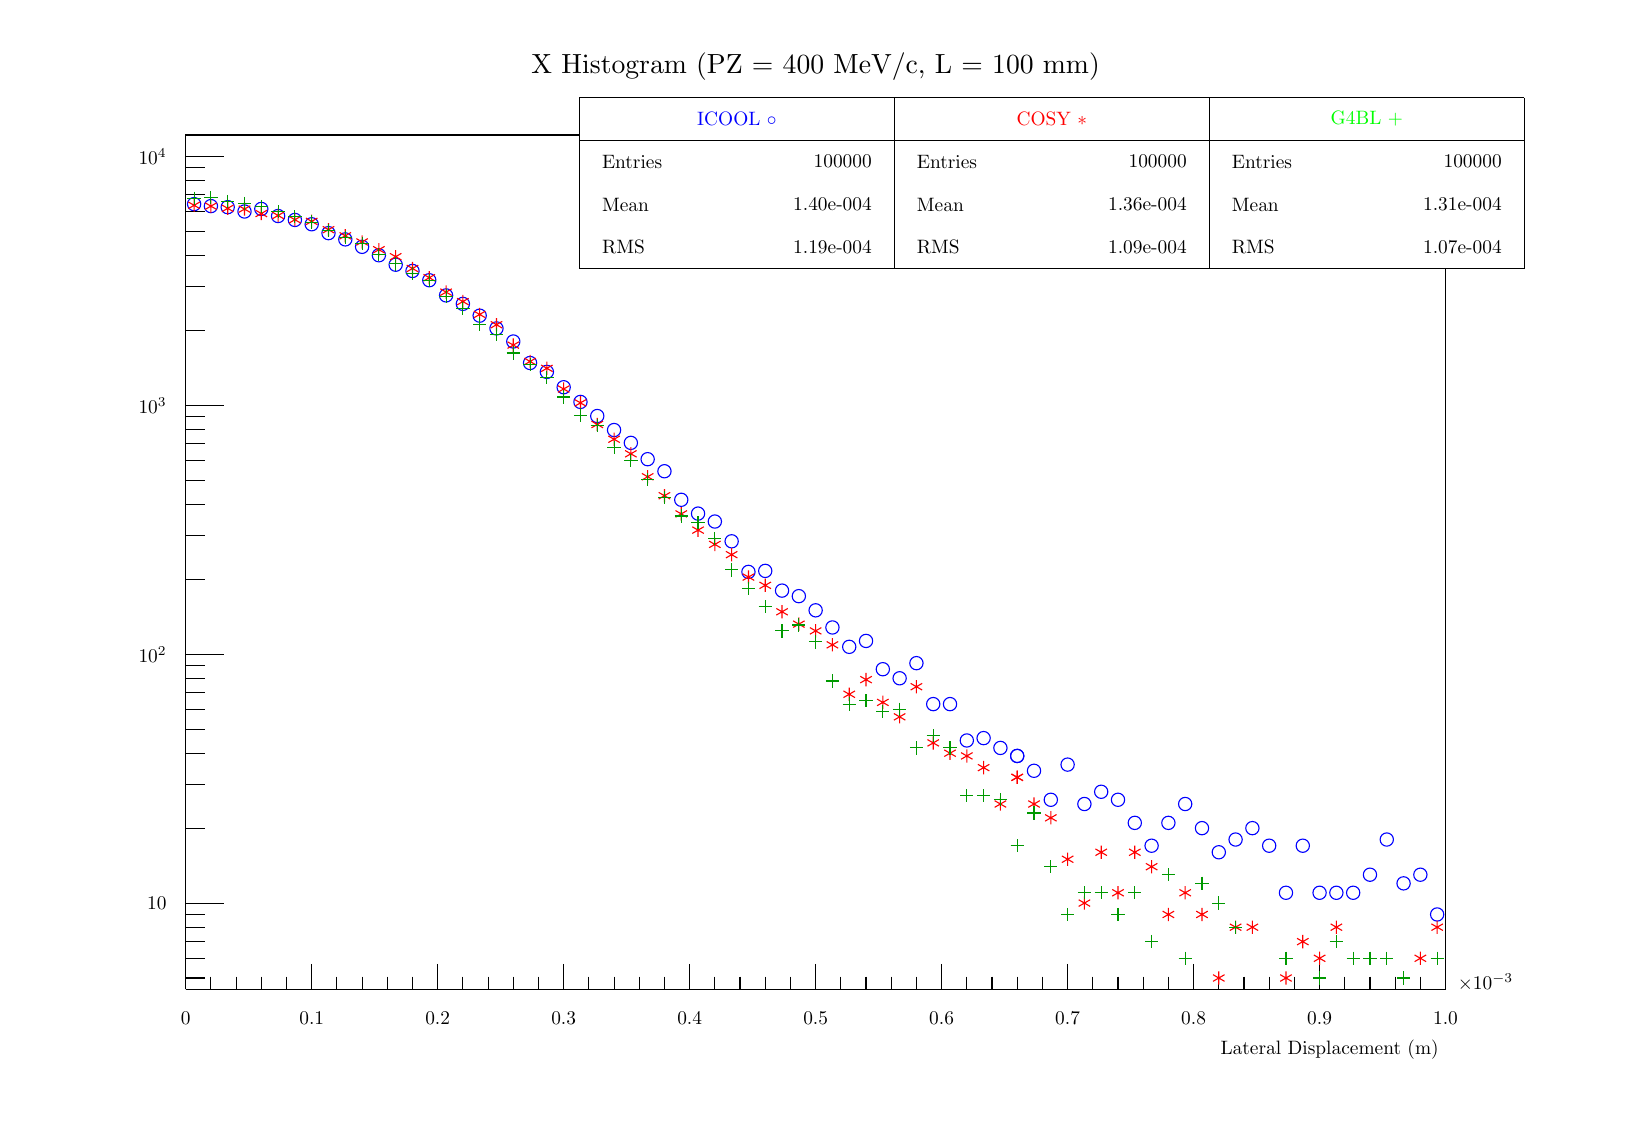
\begin{tikzpicture}
\definecolor{c}{rgb}{1,1,1};
\draw [color=c, fill=c] (0,0) rectangle (20,13.5632);
\draw [color=c, fill=c] (2,1.35632) rectangle (18,12.2069);
\definecolor{c}{rgb}{0,0,0};
\draw [c] (2,1.35632) -- (2,12.2069) -- (18,12.2069) -- (18,1.35632) -- (2,1.35632);
\definecolor{c}{rgb}{1,1,1};
\draw [color=c, fill=c] (2,1.35632) rectangle (18,12.2069);
\definecolor{c}{rgb}{0,0,0};
\draw [c] (2,1.35632) -- (2,12.2069) -- (18,12.2069) -- (18,1.35632) -- (2,1.35632);
\definecolor{c}{rgb}{0,0,1};
\foreach \P in
 {(2.10667,11.3295),(2.32,11.3043),(2.53333,11.2909),(2.74667,11.2356),(2.96,11.2681),(3.17333,11.1781),(3.38667,11.1283),(3.6,11.0736),(3.81333,10.9607),(4.02667,10.8813),(4.24,10.7869),(4.45333,10.6798),(4.66667,10.5598),(4.88,10.4805),(5.09333,10.
3626),(5.30667,10.17),(5.52,10.0625),(5.73333,9.91269),(5.94667,9.75061),(6.16,9.58443),(6.37333,9.31154),(6.58667,9.19832),(6.8,9.00356),(7.01333,8.81707),(7.22667,8.63811),(7.44,8.46019),(7.65333,8.29719),(7.86667,8.08976),(8.08,7.93679),(8.29333,7
.5743),(8.50667,7.39895),(8.72,7.29806),(8.93333,7.04695),(9.14667,6.65841),(9.36,6.67118),(9.57333,6.42087),(9.78667,6.35045),(10,6.17056),(10.2133,5.9528),(10.4267,5.70677),(10.64,5.78168),(10.8533,5.42269),(11.0667,5.30752),(11.28,5.49941),(11.493
3,4.97954),(11.7067,4.97954),(11.92,4.51759),(12.1333,4.54777),(12.3467,4.42287),(12.56,4.32113)}{\draw[mark options={color=c,fill=c},mark size=2.402402pt,mark=o] plot coordinates {\P};}
\foreach \P in
 {(12.56,4.32113),(12.7733,4.13276),(12.9867,3.76445),(13.2,4.21123),(13.4133,3.71061),(13.6267,3.8662),(13.84,3.76445),(14.0533,3.47123),(14.2667,3.18112),(14.48,3.47123),(14.6933,3.71061),(14.9067,3.40425),(15.12,3.09789),(15.3333,3.2596),(15.5467,
3.40425),(15.76,3.18112),(15.9733,2.58346),(16.1867,3.18112),(16.4,2.58346),(16.6133,2.58346),(16.8267,2.58346),(17.04,2.81282),(17.2533,3.2596),(17.4667,2.70292),(17.68,2.81282),(17.8933,2.30796)}{\draw[mark options={color=c,fill=c},mark
 size=2.402402pt,mark=o] plot coordinates {\P};}
\definecolor{c}{rgb}{1,1,1};
\draw [color=c, fill=c] (7,10.5115) rectangle (11,12.6816);
\definecolor{c}{rgb}{0,0,0};
\draw [c] (7,10.5115) -- (11,10.5115);
\draw [c] (11,10.5115) -- (11,12.6816);
\draw [c] (11,12.6816) -- (7,12.6816);
\draw [c] (7,12.6816) -- (7,10.5115);
\draw[color=blue](9,12.4103) node[scale=0.7, rotate=0]{ICOOL $\circ$};
\draw [c] (7,12.1391) -- (11,12.1391);
\draw [anchor= west] (7.2,11.8678) node[scale=0.7, rotate=0]{Entries };
\draw [anchor= east] (10.8,11.8678) node[scale=0.7, rotate=0]{ 100000};
\draw [anchor= west] (7.2,11.3253) node[scale=0.7, rotate=0]{Mean  };
\draw [anchor= east] (10.8,11.3253) node[scale=0.7, rotate=0]{ 1.40e-004};
\draw [anchor= west] (7.2,10.7828) node[scale=0.7, rotate=0]{RMS   };
\draw [anchor= east] (10.8,10.7828) node[scale=0.7, rotate=0]{ 1.19e-004};
\draw [c] (2,1.35632) -- (18,1.35632);
\draw [anchor= east] (18,0.596782) node[scale=0.7, rotate=0]{Lateral Displacement (m)};
\draw [c] (2,1.68184) -- (2,1.35632);
\draw [c] (2.32,1.51908) -- (2.32,1.35632);
\draw [c] (2.64,1.51908) -- (2.64,1.35632);
\draw [c] (2.96,1.51908) -- (2.96,1.35632);
\draw [c] (3.28,1.51908) -- (3.28,1.35632);
\draw [c] (3.6,1.68184) -- (3.6,1.35632);
\draw [c] (3.92,1.51908) -- (3.92,1.35632);
\draw [c] (4.24,1.51908) -- (4.24,1.35632);
\draw [c] (4.56,1.51908) -- (4.56,1.35632);
\draw [c] (4.88,1.51908) -- (4.88,1.35632);
\draw [c] (5.2,1.68184) -- (5.2,1.35632);
\draw [c] (5.52,1.51908) -- (5.52,1.35632);
\draw [c] (5.84,1.51908) -- (5.84,1.35632);
\draw [c] (6.16,1.51908) -- (6.16,1.35632);
\draw [c] (6.48,1.51908) -- (6.48,1.35632);
\draw [c] (6.8,1.68184) -- (6.8,1.35632);
\draw [c] (7.12,1.51908) -- (7.12,1.35632);
\draw [c] (7.44,1.51908) -- (7.44,1.35632);
\draw [c] (7.76,1.51908) -- (7.76,1.35632);
\draw [c] (8.08,1.51908) -- (8.08,1.35632);
\draw [c] (8.4,1.68184) -- (8.4,1.35632);
\draw [c] (8.72,1.51908) -- (8.72,1.35632);
\draw [c] (9.04,1.51908) -- (9.04,1.35632);
\draw [c] (9.36,1.51908) -- (9.36,1.35632);
\draw [c] (9.68,1.51908) -- (9.68,1.35632);
\draw [c] (10,1.68184) -- (10,1.35632);
\draw [c] (10.32,1.51908) -- (10.32,1.35632);
\draw [c] (10.64,1.51908) -- (10.64,1.35632);
\draw [c] (10.96,1.51908) -- (10.96,1.35632);
\draw [c] (11.28,1.51908) -- (11.28,1.35632);
\draw [c] (11.6,1.68184) -- (11.6,1.35632);
\draw [c] (11.92,1.51908) -- (11.92,1.35632);
\draw [c] (12.24,1.51908) -- (12.24,1.35632);
\draw [c] (12.56,1.51908) -- (12.56,1.35632);
\draw [c] (12.88,1.51908) -- (12.88,1.35632);
\draw [c] (13.2,1.68184) -- (13.2,1.35632);
\draw [c] (13.52,1.51908) -- (13.52,1.35632);
\draw [c] (13.84,1.51908) -- (13.84,1.35632);
\draw [c] (14.16,1.51908) -- (14.16,1.35632);
\draw [c] (14.48,1.51908) -- (14.48,1.35632);
\draw [c] (14.8,1.68184) -- (14.8,1.35632);
\draw [c] (15.12,1.51908) -- (15.12,1.35632);
\draw [c] (15.44,1.51908) -- (15.44,1.35632);
\draw [c] (15.76,1.51908) -- (15.76,1.35632);
\draw [c] (16.08,1.51908) -- (16.08,1.35632);
\draw [c] (16.4,1.68184) -- (16.4,1.35632);
\draw [c] (16.72,1.51908) -- (16.72,1.35632);
\draw [c] (17.04,1.51908) -- (17.04,1.35632);
\draw [c] (17.36,1.51908) -- (17.36,1.35632);
\draw [c] (17.68,1.51908) -- (17.68,1.35632);
\draw [c] (18,1.68184) -- (18,1.35632);
\draw [anchor=base] (2,0.908736) node[scale=0.7, rotate=0]{0};
\draw [anchor=base] (3.6,0.908736) node[scale=0.7, rotate=0]{0.1};
\draw [anchor=base] (5.2,0.908736) node[scale=0.7, rotate=0]{0.2};
\draw [anchor=base] (6.8,0.908736) node[scale=0.7, rotate=0]{0.3};
\draw [anchor=base] (8.4,0.908736) node[scale=0.7, rotate=0]{0.4};
\draw [anchor=base] (10,0.908736) node[scale=0.7, rotate=0]{0.5};
\draw [anchor=base] (11.6,0.908736) node[scale=0.7, rotate=0]{0.6};
\draw [anchor=base] (13.2,0.908736) node[scale=0.7, rotate=0]{0.7};
\draw [anchor=base] (14.8,0.908736) node[scale=0.7, rotate=0]{0.8};
\draw [anchor=base] (16.4,0.908736) node[scale=0.7, rotate=0]{0.9};
\draw [anchor=base] (18,0.908736) node[scale=0.7, rotate=0]{1.0};
\draw [anchor=base west] (18.07,1.35632) node[scale=0.7, rotate=0]{$\times10^{-3}$};
\draw [c] (2,1.35632) -- (2,12.2069);
\draw [c] (2.24,1.50097) -- (2,1.50097);
\draw [c] (2.24,1.75128) -- (2,1.75128);
\draw [c] (2.24,1.96292) -- (2,1.96292);
\draw [c] (2.24,2.14625) -- (2,2.14625);
\draw [c] (2.24,2.30796) -- (2,2.30796);
\draw [c] (2.48,2.45261) -- (2,2.45261);
\draw [anchor= east] (1.844,2.45261) node[scale=0.7, rotate=0]{10};
\draw [c] (2.24,3.40425) -- (2,3.40425);
\draw [c] (2.24,3.96092) -- (2,3.96092);
\draw [c] (2.24,4.35588) -- (2,4.35588);
\draw [c] (2.24,4.66224) -- (2,4.66224);
\draw [c] (2.24,4.91256) -- (2,4.91256);
\draw [c] (2.24,5.12419) -- (2,5.12419);
\draw [c] (2.24,5.30752) -- (2,5.30752);
\draw [c] (2.24,5.46923) -- (2,5.46923);
\draw [c] (2.48,5.61388) -- (2,5.61388);
\draw [anchor= east] (1.844,5.61388) node[scale=0.7, rotate=0]{$10^{2}$};
\draw [c] (2.24,6.56552) -- (2,6.56552);
\draw [c] (2.24,7.12219) -- (2,7.12219);
\draw [c] (2.24,7.51716) -- (2,7.51716);
\draw [c] (2.24,7.82352) -- (2,7.82352);
\draw [c] (2.24,8.07383) -- (2,8.07383);
\draw [c] (2.24,8.28547) -- (2,8.28547);
\draw [c] (2.24,8.46879) -- (2,8.46879);
\draw [c] (2.24,8.6305) -- (2,8.6305);
\draw [c] (2.48,8.77515) -- (2,8.77515);
\draw [anchor= east] (1.844,8.77515) node[scale=0.7, rotate=0]{$10^{3}$};
\draw [c] (2.24,9.72679) -- (2,9.72679);
\draw [c] (2.24,10.2835) -- (2,10.2835);
\draw [c] (2.24,10.6784) -- (2,10.6784);
\draw [c] (2.24,10.9848) -- (2,10.9848);
\draw [c] (2.24,11.2351) -- (2,11.2351);
\draw [c] (2.24,11.4467) -- (2,11.4467);
\draw [c] (2.24,11.6301) -- (2,11.6301);
\draw [c] (2.24,11.7918) -- (2,11.7918);
\draw [c] (2.48,11.9364) -- (2,11.9364);
\draw [anchor= east] (1.844,11.9364) node[scale=0.7, rotate=0]{$10^{4}$};
\definecolor{c}{rgb}{1,1,1};
\draw [color=c, fill=c] (7,10.5115) rectangle (11,12.6816);
\definecolor{c}{rgb}{0,0,0};
\draw [c] (7,10.5115) -- (11,10.5115);
\draw [c] (11,10.5115) -- (11,12.6816);
\draw [c] (11,12.6816) -- (7,12.6816);
\draw [c] (7,12.6816) -- (7,10.5115);
\draw[color=blue](9,12.4103) node[scale=0.7, rotate=0]{ICOOL $\circ$};
\draw [c] (7,12.1391) -- (11,12.1391);
\draw [anchor= west] (7.2,11.8678) node[scale=0.7, rotate=0]{Entries };
\draw [anchor= east] (10.8,11.8678) node[scale=0.7, rotate=0]{ 100000};
\draw [anchor= west] (7.2,11.3253) node[scale=0.7, rotate=0]{Mean  };
\draw [anchor= east] (10.8,11.3253) node[scale=0.7, rotate=0]{ 1.40e-004};
\draw [anchor= west] (7.2,10.7828) node[scale=0.7, rotate=0]{RMS   };
\draw [anchor= east] (10.8,10.7828) node[scale=0.7, rotate=0]{ 1.19e-004};
\draw (10,13.0816) node[scale=1, rotate=0]{X Histogram (PZ = 400 MeV/c, L = 100 mm)};
\definecolor{c}{rgb}{1,0,0};
\foreach \P in
 {(2.10667,11.314),(2.32,11.3036),(2.53333,11.2755),(2.74667,11.2661),(2.96,11.2097),(3.17333,11.1848),(3.38667,11.131),(3.6,11.1099),(3.81333,11.0044),(4.02667,10.9273),(4.24,10.849),(4.45333,10.7506),(4.66667,10.6619),(4.88,10.5115),(5.09333,10.394
6),(5.30667,10.2116),(5.52,10.0917),(5.73333,9.92819),(5.94667,9.7977),(6.16,9.53875),(6.37333,9.33091),(6.58667,9.24395),(6.8,8.98129),(7.01333,8.80503),(7.22667,8.53087),(7.44,8.34308),(7.65333,8.15814),(7.86667,7.86676),(8.08,7.62599),(8.29333,7.3
952),(8.50667,7.18918),(8.72,7.00772),(8.93333,6.87736),(9.14667,6.59271),(9.36,6.48785),(9.57333,6.15213),(9.78667,5.99505),(10,5.90921),(10.2133,5.7322),(10.4267,5.10444),(10.64,5.29025),(10.8533,5.00117),(11.0667,4.81784),(11.28,5.20049),(11.4933,
4.48674),(11.7067,4.35589),(11.92,4.32113),(12.1333,4.17256),(12.3467,3.71061),(12.56,4.04953)}{\draw[mark options={color=c,fill=c},mark size=2.402402pt,mark=asterisk] plot coordinates {\P};}
\foreach \P in
 {(12.56,4.04953),(12.7733,3.71061),(12.9867,3.5351),(13.2,3.00928),(13.4133,2.45261),(13.6267,3.09789),(13.84,2.58346),(14.0533,3.09789),(14.2667,2.91456),(14.48,2.30796),(14.6933,2.58346),(14.9067,2.30796),(15.12,1.50097),(15.3333,2.14625),(15.5467
,2.14625),(15.9733,1.50097),(16.1867,1.96292),(16.4,1.75129),(16.6133,2.14625),(17.68,1.75129),(17.8933,2.14625)}{\draw[mark options={color=c,fill=c},mark size=2.402402pt,mark=asterisk] plot coordinates {\P};}
\definecolor{c}{rgb}{1,1,1};
\draw [color=c, fill=c] (11,10.5115) rectangle (15,12.6816);
\definecolor{c}{rgb}{0,0,0};
\draw [c] (11,10.5115) -- (15,10.5115);
\draw [c] (15,10.5115) -- (15,12.6816);
\draw [c] (15,12.6816) -- (11,12.6816);
\draw [c] (11,12.6816) -- (11,10.5115);
\draw [color=red](13,12.4103) node[scale=0.7, rotate=0]{COSY $*$};
\draw [c] (11,12.1391) -- (15,12.1391);
\draw [anchor= west] (11.2,11.8678) node[scale=0.7, rotate=0]{Entries };
\draw [anchor= east] (14.8,11.8678) node[scale=0.7, rotate=0]{ 100000};
\draw [anchor= west] (11.2,11.3253) node[scale=0.7, rotate=0]{Mean  };
\draw [anchor= east] (14.8,11.3253) node[scale=0.7, rotate=0]{ 1.36e-004};
\draw [anchor= west] (11.2,10.7828) node[scale=0.7, rotate=0]{RMS   };
\draw [anchor= east] (14.8,10.7828) node[scale=0.7, rotate=0]{ 1.09e-004};
\definecolor{c}{rgb}{1,1,1};
\draw [color=c, fill=c] (11,10.5115) rectangle (15,12.6816);
\definecolor{c}{rgb}{0,0,0};
\draw [c] (11,10.5115) -- (15,10.5115);
\draw [c] (15,10.5115) -- (15,12.6816);
\draw [c] (15,12.6816) -- (11,12.6816);
\draw [c] (11,12.6816) -- (11,10.5115);
\draw [color=red](13,12.4103) node[scale=0.7, rotate=0]{COSY $*$};
\draw [c] (11,12.1391) -- (15,12.1391);
\draw [anchor= west] (11.2,11.8678) node[scale=0.7, rotate=0]{Entries };
\draw [anchor= east] (14.8,11.8678) node[scale=0.7, rotate=0]{ 100000};
\draw [anchor= west] (11.2,11.3253) node[scale=0.7, rotate=0]{Mean  };
\draw [anchor= east] (14.8,11.3253) node[scale=0.7, rotate=0]{ 1.36e-004};
\draw [anchor= west] (11.2,10.7828) node[scale=0.7, rotate=0]{RMS   };
\draw [anchor= east] (14.8,10.7828) node[scale=0.7, rotate=0]{ 1.09e-004};
\definecolor{c}{rgb}{0,0.6,0};
\foreach \P in
 {(2.10667,11.4047),(2.32,11.4124),(2.53333,11.363),(2.74667,11.3361),(2.96,11.2993),(3.17333,11.2328),(3.38667,11.1692),(3.6,11.1008),(3.81333,10.9963),(4.02667,10.9068),(4.24,10.8263),(4.45333,10.687),(4.66667,10.5699),(4.88,10.4513),(5.09333,10.35
65),(5.30667,10.161),(5.52,10.0054),(5.73333,9.8055),(5.94667,9.67717),(6.16,9.43834),(6.37333,9.29378),(6.58667,9.12476),(6.8,8.87954),(7.01333,8.65019),(7.22667,8.51603),(7.44,8.2396),(7.65333,8.07383),(7.86667,7.83446),(8.08,7.60684),(8.29333,7.36
869),(8.50667,7.28186),(8.72,7.08037),(8.93333,6.68384),(9.14667,6.45104),(9.36,6.21557),(9.57333,5.90921),(9.78667,5.98461),(10,5.76947),(10.2133,5.27276),(10.4267,4.97954),(10.64,5.02245),(10.8533,4.88948),(11.0667,4.91256),(11.28,4.42287),(11.4933
,4.5773),(11.7067,4.42287),(11.92,3.81627),(12.1333,3.81627),(12.3467,3.76445),(12.56,3.18112)}{\draw[mark options={color=c,fill=c},mark size=2.402402pt,mark=+] plot coordinates {\P};}
\foreach \P in
 {(12.56,3.18112),(12.7733,3.59613),(12.9867,2.91456),(13.2,2.30796),(13.4133,2.58346),(13.6267,2.58346),(13.84,2.30796),(14.0533,2.58346),(14.2667,1.96292),(14.48,2.81282),(14.6933,1.75129),(14.9067,2.70292),(15.12,2.45261),(15.3333,2.14625),(15.973
3,1.75129),(16.4,1.50097),(16.6133,1.96292),(16.8267,1.75129),(17.04,1.75129),(17.2533,1.75129),(17.4667,1.50097),(17.8933,1.75129)}{\draw[mark options={color=c,fill=c},mark size=2.402402pt,mark=+] plot coordinates {\P};}
\definecolor{c}{rgb}{1,1,1};
\draw [color=c, fill=c] (15,10.5115) rectangle (19,12.6816);
\definecolor{c}{rgb}{0,0,0};
\draw [c] (15,10.5115) -- (19,10.5115);
\draw [c] (19,10.5115) -- (19,12.6816);
\draw [c] (19,12.6816) -- (15,12.6816);
\draw [c] (15,12.6816) -- (15,10.5115);
\draw [color=green](17,12.4103) node[scale=0.7, rotate=0]{G4BL $+$};
\draw [c] (15,12.1391) -- (19,12.1391);
\draw [anchor= west] (15.2,11.8678) node[scale=0.7, rotate=0]{Entries };
\draw [anchor= east] (18.8,11.8678) node[scale=0.7, rotate=0]{ 100000};
\draw [anchor= west] (15.2,11.3253) node[scale=0.7, rotate=0]{Mean  };
\draw [anchor= east] (18.8,11.3253) node[scale=0.7, rotate=0]{ 1.31e-004};
\draw [anchor= west] (15.2,10.7828) node[scale=0.7, rotate=0]{RMS   };
\draw [anchor= east] (18.8,10.7828) node[scale=0.7, rotate=0]{ 1.07e-004};
\definecolor{c}{rgb}{1,1,1};
\draw [color=c, fill=c] (15,10.5115) rectangle (19,12.6816);
\definecolor{c}{rgb}{0,0,0};
\draw [c] (15,10.5115) -- (19,10.5115);
\draw [c] (19,10.5115) -- (19,12.6816);
\draw [c] (19,12.6816) -- (15,12.6816);
\draw [c] (15,12.6816) -- (15,10.5115);
\draw [color=green](17,12.4103) node[scale=0.7, rotate=0]{G4BL $+$};
\draw [c] (15,12.1391) -- (19,12.1391);
\draw [anchor= west] (15.2,11.8678) node[scale=0.7, rotate=0]{Entries };
\draw [anchor= east] (18.8,11.8678) node[scale=0.7, rotate=0]{ 100000};
\draw [anchor= west] (15.2,11.3253) node[scale=0.7, rotate=0]{Mean  };
\draw [anchor= east] (18.8,11.3253) node[scale=0.7, rotate=0]{ 1.31e-004};
\draw [anchor= west] (15.2,10.7828) node[scale=0.7, rotate=0]{RMS   };
\draw [anchor= east] (18.8,10.7828) node[scale=0.7, rotate=0]{ 1.07e-004};
\end{tikzpicture}
